\documentclass[a4paper, 12pt, one column, aas_macros]{article}

%% Language and font encodings. This says how to do hyphenation on end of lines.
\usepackage[english]{babel}
%\usepackage[utf8x]{inputenc}
\usepackage[T1]{fontenc}
\usepackage{aas_macros}

%% Sets page size and margins. You can edit this to your liking
\usepackage[top=1.3cm, bottom=2.0cm, outer=2.5cm, inner=2.5cm, heightrounded, marginparwidth=1.5cm, marginparsep=0.4cm, margin=2.5cm]{geometry}

%% Useful packages
\usepackage{graphicx} %allows you to use jpg or png images. PDF is still recommended
\usepackage[colorlinks=False]{hyperref} % add links inside PDF files
\usepackage{amsmath}  % Math fonts
\usepackage{amsfonts} %
\usepackage{amssymb}  %
\usepackage{tikz}
\usepackage{float}
\usepackage{indentfirst}
\usetikzlibrary{quantikz}

%% Citation package
\usepackage[authoryear]{natbib}
\bibliographystyle{abbrvnat}
\setcitestyle{authoryear,open={},close={}}
\setlength{\parindent}{1em}
\title{Option Pricing using Canonical Amplitude Estimation}
\author{Constantin Kurz \\ Thomas Jung \\ Deepankar Bhagat}
\begin{document}
\maketitle

\section{Introduction}
In this work we will present how to compute the pricing of an option on a quantum computer and compare this with a classical Monte Carlo simulation.
We go over the steps to build a call option on a gate-based quantum computer, for example the IBM Q Tokyo. We use qiskit (\cite{Qiskit}) a python module to connect the gates and qubits and simulate the result.
Therefor we try to rebuild the logic of the gate-based quantum computer described in this paper \cite{1905.02666}.

BLABLABLABLABLA.
\bibliography{./refs}
\section{Black-Scholes-Merton-Model and European Call Options}

The Black-Scholes-Merton (BSM) model considers the pricing of financial derivatives (‘options’). The original model assumes a single benchmark asset (‘stock’), the price of which is stochastically driven by a Brownian motion, see fig $\ref{fig:stockPaths}$. In addition, it assumes a risk-free investment into a bank account (‘bond’).\\
The Black-Scholes-Merton model consists of two assets, one risky (the stock), the other one risk-free (the bond). The risky asset is defined by the stochastic differential equation for the price dynamics given by
\begin{equation}
    dS_t = S_t r dt + S_t \sigma dW_t,
\end{equation}
where $r$ is the drift, $\sigma$ the volatility and dWt is a Brownian increment. The initial condition is S0. In addition, the risk-free asset dynamics is given by
\begin{equation}
   dB_t = B_t r dt, 
\end{equation}
where r is the risk-free rate (market rate).\\
the risky asset stochastic differential equation can be solved as
\begin{align}
	   S_i &=S_{0}\cdot\exp^{\sigma \cdot W_i+(r-\frac{\sigma^2}{2})T} \label{eq:S_T} \\
	   W_i &= \mathcal{N}(\mu=0,\sigma^2=T) \label{eq:W_T}.
\end{align}
The risk-free asset is solved easily as
\begin{equation}
    B_t = e^{rt}.
\end{equation}
This risk-free asset also is used for ‘discounting’, i.e. determining the present value of a future amount of money.
One of the simplest options is the European call option. The European call option gives the owner of the option the right to buy the stock at maturity time $T \geq 0$ for a pre-agreed strike price $K$.\\
The payoff is defined as
\begin{equation}
    f(S_T) = \max(0, S_T - K ).
\end{equation}
The task of pricing is to evaluate at present time $t = 0$ the expectation value of the option $f(S_T)$ on the stock on the maturity date.
The pricing problem is thus given by evaluating the risk-neutral price
\begin{equation}
    \Pi = e^{-rt} \mathbb{E}[f(S_T)],
\end{equation}
where $e^{-rT}$ is the discount factor, which determines the present value of the payoff at a future time, given the model assumption of a risk-free asset growing with r.\\
The asset price a maturity $T$ follows a log-normal distribution wit probability density (\cite{1905.02666})
\begin{equation}
    P(S_T) = \frac{1}{S_T \sigma \sqrt{2 \pi T}} exp (- \frac{(\text{ln} S_T - \mu)^2}{2 \sigma^2 T}, \label{eq:lognormal}
\end{equation}
where $\sigma$ is the volatility of the asset and $\mu = (r-0.5\sigma^2)T + \text{ln}(S_0)$.
\bibliography{./refs}

\section{Monte Carlo Simulation}    
In this section we discuss how Monte Carlo Simulations are working and compare them to quantum computer.
\subsection{Classic Monte Carlo}
\subsubsection{Theory} \label{sec:classic_mc_theory}
In general monte carlo data are generated if an experiment or an calculation doesn't have sufficient training data. To generate data using the Monte Carlo method we can following these steps (\cite{1905.02666}):
\begin{enumerate}
	\item At first we need a set of random variables $\textbf{X}=\{X_1, X_2, \dots, X_N\}$. In our case this values describe the asset price and other sources of uncertainties.
	\item With this information's we can now create additional information. In our case we can build $M$ random price paths $\{ \textbf{X}_1, \textbf{X}_2, \dots, \textbf{X}_N \}$ .
	\item At the end we want to have the expected value of the payoff $\mathbb{E}_P$, for this we can calculate the payoff of every path $F(\textbf{X}_i)$ and then build the average of the results:
	    \begin{align}
	        \mathbb{E}_P[F(\textbf{X})] = \frac{1}{M} \sum_{i=1}^{M} F(\textbf{X}_i)
	    \end{align}
\end{enumerate}

In this work we will use the "Black-Scholes-Merton" model to create the paths of the stock price. After the Black-Scholes-Merton method the value of the stock changes each step after a log-normal distribution shown in figure \ref{fig:stockPaths}.

To calculate the end result we split the time frame $T$ in $n$ steps, with each step the size of $dt=\frac{T}{n}$. We need also the volatility $\sigma$ and the drift $r$ of the stock.
\begin{figure}[H]
  \begin{center}
    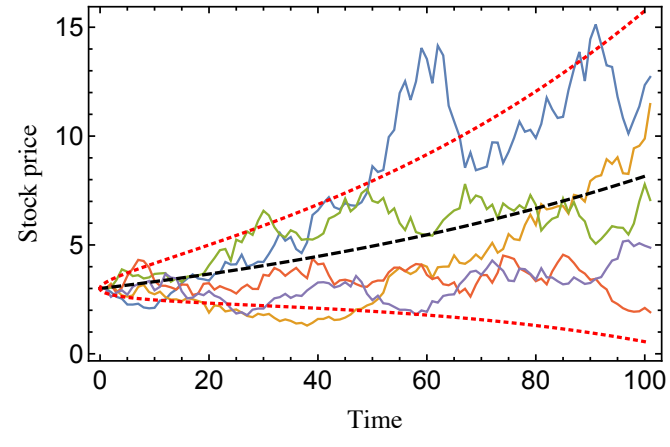
\includegraphics[width=0.5\linewidth]{images/stock_path.png}
  \end{center}
  \caption{Image of five different paths of the stock price. The stock price is in dollar and the time is in days. The dashed black line is the mean of the samples and the dotted red lines are the first standard deviation. The parameters are: $S_0=\$3, r=0.1, \sigma=0.25$ \cite{1805.00109}}
  \label{fig:stockPaths}
\end{figure}
Now $\Pi$ is the true option price and $\hat{\Pi}$ is the approximation of the option price calculated via the Monte Carlo data, with $M$ samples. With this values and the condition that the variance of the payoff function is $ \leq \lambda^2$ the probability that $|\Pi-\hat{\Pi}| \leq \epsilon$ can be determined by Chebyshev’s inequality (\cite{1504.06987}).
\begin{align}
	        P[|\Pi-\hat{\Pi}| \leq \epsilon] \leq \frac{\lambda^2}{M\epsilon^2}
	    \end{align}
So to achieve an error of $\epsilon$
\begin{align}
	        M=\mathcal{O}(\frac{\lambda^2}{\epsilon^2}) \label{eq:classic_M}
	    \end{align}
samples are needed. Section \ref{sec:MC_quanten} shows that quantum computer can improve this from $\epsilon^2$ to $\epsilon$.

\subsubsection{Example} \label{seq:MC_example}
In this subsection a easy Monte Carlo method is shown. Therefor we create only four different stock path and only the last value is of interest, so we get this values:
\begin{align}
    \{\textbf{X}_1=1.5, \textbf{X}_2=2.3, \textbf{X}_3=2.8, \textbf{X}_4=2.11\} \nonumber
\end{align}
We use $S_0=2$ as initial value, $K=2.1$ as strike price and this
\begin{align}
    F(\textbf{X}_i) = \max\{0, X_i - K\} \label{eq:MC_example_european}
\end{align}
as the payoff function. With this kind of information's we can now calculate our expected payoff
\begin{align}
    \mathbb{E}_P[F(\textbf{X})] &= \frac{1}{4}(0+0.01+0.2+0.7 ) \nonumber \\
    &= 0.2275 \nonumber
\end{align}
\bibliography{././refs}
\subsection{Quantum Monte Carlo Simulations\label{sec:MC_quanten}
In the quantum field three problems has to be solved. (\cite{1905.02666})
\begin{enumerate}
	\item Load the probability Estimation (the log-normal distribution) in to the quantum computer. This problem is described in section \ref{sec:MC_QGAN}
	\item The payoff function $F(\textbf{X})$ has to be build with qubits inside the quantum computer. In section \ref{sec:MC_Payoff} the payoff function is constructed.
	\item The quantum computer should calculate at the end the expected value of the payoff $\mathbb{E}_P[F(\textbf{X})]$, this will also be explained in section \ref{sec:MC_Payoff}.
\end{enumerate}
But before we can describe how to construct the gates to build the payoff function, we need to explain how amplitude estimation is working in an quantum computer. We are doing this in section \ref{sec:MC_AE}

\subsubsection{Loading the distribution (QuGAN)}\label{sec:MC_QGAN}
In this section we go over the basics of the QuGAN, because we use an already implemented function, which is not QuGAN, of qiskit (\cite{Qiskit}) later to load in the log-normal distribution.

QuGAN stands for Quantum Generative Adversarial Networks and it creates fake data which are similar to the real data. The GAN method is used when there are only a few real world data or to bring the data in to a new system. The last one is exactly our purpose here. We want to have the log-normal distribution inside a quantum computer. For this we divide the log-normal distribution in distinct buckets $n$. The value of $n$ has to be the number of states the $k$ qubits can have $n=2^{k}$. So if we have 3 qubits we have 8 distinct buckets. Every state of all the $k$ qubits maps to a real value.

The structure of an QuGAN is shown in figure \ref{fig:qgan}. So a QuGAN goes throw this steps:
\begin{enumerate}
	\item We load in at first the classical dataset, transform the Dateset and with this dataset initial parameter for the gates can be created.
	\item With this parameters the quantum circuit can be created. \label{enu:QuGan_parameter}
	\item The quantum circuit is then loaded into a quantum computer.
	\item After optimise steps in the quantum computer the quantum state is measured.
	\item The quantum state is then transformed in to the classical world and the loss is calculated. Also the Quantum Circuits can create sample states and this sample states are then used to generate classical data points.
	\item With the loss the parameters of the circuit can be update. After updating the circuits parameter we go back to step \ref{enu:QuGan_parameter}.
\end{enumerate}
\begin{figure}[H]
  \begin{center}
    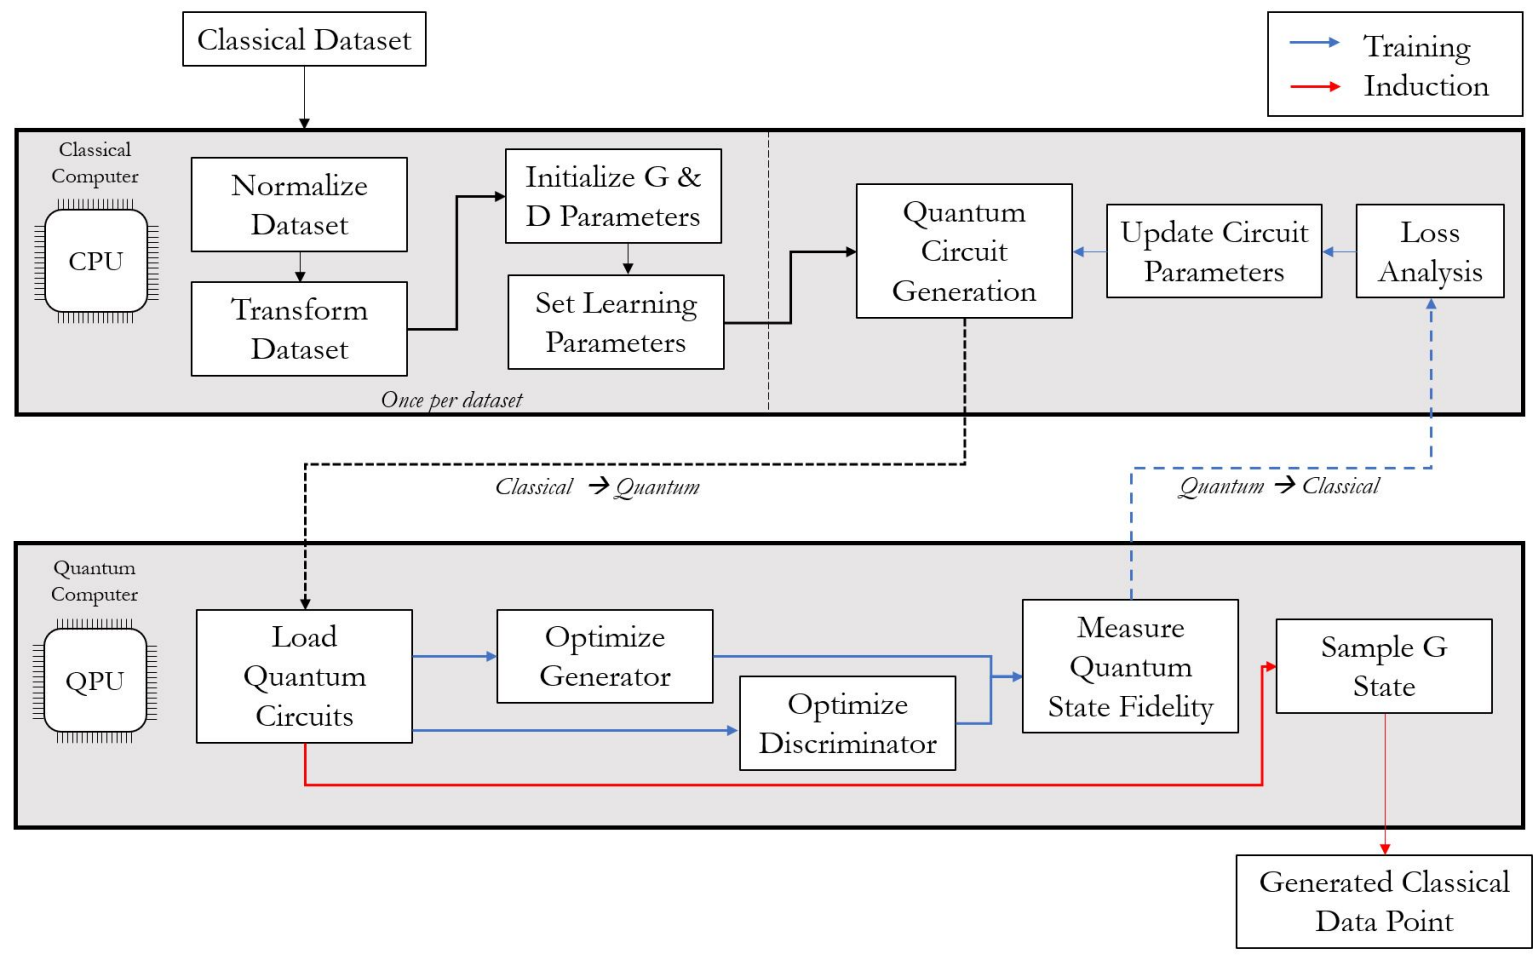
\includegraphics[width=\linewidth]{images/qgan_structure.png}
  \end{center}
  \caption{ QuGAN System Architecture \cite{2010.09036}}
  \label{fig:qgan}
\end{figure}
\subsubsection{Amplitude Estimation}\label{sec:MC_AE}
For the Amplitude Estimation (AE) we need an unitary operator $A$ which behaves on an register of $(n+1)$ qubits like this
\begin{align}
    A\ket{0}_{n+1} &= \sqrt{1-a}\ket{\psi_0}_{n}\ket{0}+\sqrt{a}\ket{\psi_1}_{n}\ket{1}. \label{eq:AE_A}
\end{align}

In the equation \ref{eq:AE_A} $\ket{\psi_0}_{n}$ and $\ket{\psi_1}_{n}$ are some normalized states and $a$ is a unknown variable $\in [0,1]$.
With Amplitude Estimation we can estimate the value of $a$ therefor we have to construct our problem so that we have this at the end $a=\mathbb{E}_P[f(\textbf{X})]$.
To make a use of $\sin$ and $\cos$ to work with RY-Gates we can say that $a=\sin^2(\theta_a)$ is, so that equation \ref{eq:AE_A} turns into this
\begin{align}
    A\ket{0}_{n+1} &= \cos(\theta_a)\ket{\psi_0}_{n}\ket{0}+\sin(\theta_a)\ket{\psi_1}_{n}\ket{1}. \label{eq:AE_A_sin} \\
    \theta_p &= 2 \theta_a \nonumber \\
    A &= R_Y(\theta_p)
\end{align}

With this changes we transformed the amplitude estimation in to a phase estimation.\\
The next step is to determine the Grover operator $\mathcal{Q}=AS_0A^\dagger S_{\psi_1}$.\\
$S_0$ is a reflection about the $\ket{0}$ state and $S_{\psi_1}$ is a reflection about the $|\psi_1>$ state. So we can write $S$ and $\mathcal{Q}$ like this:
\begin{align}
    S_0 &= 1-2\ket{0}\bra{0} \nonumber \\
    S_{\psi_1} &= 1-2\ket{\psi_1}\ket{0}\bra{\psi_1}\bra{0} \nonumber \\
    \mathcal{Q} &= R_Y(2\theta_p) \\ 
    \mathcal{Q}_{2^j} &= R_Y(2^j\cdot 2\theta_p)
\end{align}
\begin{figure}[H]
  \begin{center}
\begin{quantikz}
\lstick{(0) \ket{0}} & \gate{H} & \ctrl{5} & \ldots \qw & \qw & \ldots \qw & \qw & \gate[5, nwires={2,4}]{QFT^{\dagger}} &  \meter{}\\
 & \vdots & & \ddots & & \ddots & & \\
\lstick{(j) \ket{0}} & \gate{H} & \qw & \ldots \qw & \ctrl{3} & \ldots \qw & \qw & & \meter{}\\
 & \vdots & & \ddots & & \ddots & &\\
\lstick{(n-1) \ket{0}} & \gate{H} & \qw & \ldots \qw & \qw & \ldots \qw & \ctrl{1} & &  \meter{}\\
\lstick{(n) \ket{0}} & \gate[wires=2]{A} & \gate[wires=2]{\mathcal{Q}_{2^0}} & \ldots \qw & \gate[wires=2]{\mathcal{Q}_{2^j}} & \ldots \qw & \gate[wires=2]{\mathcal{Q}_{2^{n-1}}} & \qw\\
\lstick{(n+m-1) \ket{0}} &  & & \ldots \qw &  & \ldots \qw & & \qw
\end{quantikz}
\end{center}
\caption{ Design of the Amplitude Estimation recreated after \cite{1905.02666}}
\label{fig:qgan}
\end{figure}
The error $\epsilon$ of this method defined as followed
\begin{align}
    |\hat{\Pi} - \Pi| &\leq C\cdot(\frac{\sqrt{\mathbb{E}}}{M} + \frac{1}{M^2}) \nonumber \\
    M &= \mathcal{O}(\frac{1}{\epsilon \sqrt{\mathbb{E}}}) \label{eq:AE_M}
\end{align}
As we can see in \ref{eq:classic_M} and \ref{eq:AE_M} quantum computer improved the number error with the same number of samples
\subsubsection{Construct the payoff function}\label{sec:MC_Payoff}
A lot of payoff function can be constructed by piece-wise linear functions, in this section we will go over how to construct the piece-wise linear function in to quantum computer.

First of all we need to transform the payoff function $F(\textbf{X})$ in to new functions $f_b(i)=m_b\cdot i + o_b$, with $m_b$ the slope of the function and $o_b$ the offset of the function. For every break point $b$ of the payoff function we need to create a new function $f_b$. The new function gets the following as input $i\in\{0,\ldots, 2^n-1\}$, which represents all states the qubits can have. For example we have three qubits ($i\in\{0,1,2,3,4,5,6,7\}$) so $\ket{011}$ mapes to $i=3$. The output of the function can also only be $f(i)\in[0,1]$ this was shown in section \ref{sec:MC_AE}. Now that we build the function we can insert the function in this equation \ref{eq:AE_A_sin} and get this new equation
\begin{align}
    \ket{i}_n\ket{0} &= \ket{i}_n(\cos[f(i)]\ket{0}+\sin[f(i)]\ket{1}) \label{eq:PF_f}
\end{align}

So this function can be rebuild in a quantum computer with controlled $Y$-Rotations $CR_y$ and normal $Y$-Rotations $R_y$, the normal $Y$-Rotation is only used to initially rotate the qubit, which corresponds to the first offset. To do this we need an extra qubit on which we perform the rotations based on $x$ encoded in register $\ket{i}_n$ which is already holding the probability distribution. Similar to the Amplitude Estimation the rotations add a factor $2^{j}$, where the ${j}$'s are qubits from $\ket{i}_n$-register. (shown in figure \ref{fig:PF_y}) Consequently the more $\ket{j}$ are set to $\ket{1}$, the higher the value of $x$ is. If we add more qubits to $\ket{i}_n$-register, i.e. more grid-points, a higher accuracy can be reached.

\begin{figure}[H]
  \begin{center}
\begin{quantikz}
\lstick{\ket{q_0}} & \qw & \ctrl{3} & \qw & \qw & \qw\\
\lstick{\ket{q_1}} & \qw & \qw & \ctrl{2} & \qw & \qw\\
\lstick{\ket{q_2}} & \qw & \qw & \qw & \ctrl{1} & \qw\\
\lstick{\ket{q_3}} & \gate[1]{R_y(f_0)} & \gate[1]{CR_y(f_1)} & \gate[1]{2CR_y(f_1)} & \gate[1]{4CR_y(f_1)} & \qw
\end{quantikz}
\end{center}
\caption{ Quantum circuit for a linear function. Base image copied from \cite{1905.02666}}
\label{fig:PF_y}
\end{figure}

Until now we only showed how to implement a linear function but every piece-wise linear function applies only on specific states. Now we have to build a greater or equal operation in a quantum computer, since we are dealing with a $max$ function in eq. $\ref{eq:E_example_european}$. For this we need also $n$ qubits, one of the qubits has the result at the end. So for this operation we have $n$ data qubits $\ket{q}$ and $n$ qubits for the greater or equal operation $\ket{a}$. To build the operation we can follow this steps (example of a circuit is in figure \ref{fig:PF_max}). 
\begin{enumerate}
	\item At first we convert the breakpoint $b\in[0,2^n-1]$ in a bit representation $t$. For this we use a ceil operation on b and convert it then in a bit representation $t$. Every bit represent one qubit. If the breakpoint lies between two grid points $i$, the ceil operation ensures that the respective larger grid point is used as breakpoint for controlled application of max-operation.
	\item Now we can iterate over all the qubits. (we use here $j$ as iterate parameter)
	\begin{itemize}
	    \item if it is the first qubit $j=0$ and $t[j]=1$, we have to perform a $CX$ operation on $\ket{q_j}$ and $\ket{a_j}$.
	    \item if $t[j]=1$ an $OR$-Operation has to be done on $\ket{q_j}$ and $\ket{a_{j-1}}$ the result of the $OR$-Operation will be saved in $\ket{a_j}$
	    \item if $t[j]=0$ an $CCX$-Operation has to be done on $\ket{q_j}$, $\ket{a_{j-1}}$ and $\ket{a_j}$
    \end{itemize}
    \item Now we have in $a_{n-1}$ the result saved $\ket{0}$ if $i<b$ and $\ket{1}$ if $i\geq b$.
    \item What we have to do now is to reverse the process except that now $j\in{n-1, \ldots, 0}$ is. So we do not consider the last qubit because it saves the result. To reverse an $CX$, $CCX$ and $OR$-Operation we only have to apply the same operator again.
\end{enumerate}
\begin{figure}[H]
  \begin{center}
\begin{quantikz}
\lstick{\ket{a}} & \gate{X} & \ctrl{2} & \gate{X} &  \midstick[3,brackets=none]{$\equiv$}\qw & \ctrl{2} & \qw\\
\lstick{\ket{b}} & \gate{X} & \ctrl{1} & \gate{X} & \qw & \ctrl{1} & \qw\\
\lstick{\ket{c}} & \gate{X} &  \targ{} & \qw & \qw & \gate{OR} & \qw
\end{quantikz}
\end{center}
\caption{ Example of an $OR$-Operation on qubit $\ket{a}$ and $\ket{b}$. The result is then saved in $\ket{c}$. Base image copied from \cite{1905.02666}}
\label{fig:PF_OR}
\end{figure}

\begin{figure}[H]
  \begin{center}
\begin{quantikz}
 & & & & &  & & & & & & &  \gategroup[9,steps=7,style={dashed,rounded corners,fill=blue!20, inner xsep=2pt},background]{{Inverse for n-2 to 0}}    & & & &  &  &    \\
\lstick{\ket{q_0}} & \ctrl{4}\gategroup[5,steps=1,style={dashed,rounded corners, inner xsep=2pt}]{{t[0]=1}} & \qw & \qw & \qw & \qw & \qw  & \qw & \qw & \qw & \qw & \qw & \qw & \qw & \qw & \qw & \qw & \ctrl{4}\gategroup[5,steps=1,style={dashed,rounded corners, inner xsep=2pt}]{{t[0]=1}} & \qw  \\
\lstick{\ket{q_1}} & \qw & \qw & \ctrl{4}\gategroup[5,steps=1,style={dashed,rounded corners, inner xsep=2pt}, label style={label position=below,anchor=north,yshift=-0.2cm}]{{t[1]=0}} & \qw & \ctrl{4}\gategroup[5,steps=1,style={dashed,rounded corners, inner xsep=2pt}, label style={label position=below,anchor=north,yshift=-0.2cm}]{{t[1]=1}} & \qw & \qw & \qw & \qw & \qw & \qw & \qw & \ctrl{4}\gategroup[5,steps=1,style={dashed,rounded corners, inner xsep=2pt}, label style={label position=below,anchor=north,yshift=-0.2cm}]{{t[1]=0}} & \qw & \ctrl{4}\gategroup[5,steps=1,style={dashed,rounded corners, inner xsep=2pt}, label style={label position=below,anchor=north,yshift=-0.2cm}]{{t[1]=1}} & \qw & \qw & \qw \\
\lstick{\vdots} & & & &  & & \vdots & & & & & \vdots & & & & &  &  &    \\
\lstick{\ket{q_{n-1}}} & \qw & \qw & \qw & \qw & \qw & \qw & \qw & \ctrl{4}\gategroup[6,steps=1,style={dashed,rounded corners, inner xsep=2pt}]{{t[n-1]=0}} & \qw & \ctrl{4}\gategroup[6,steps=1,style={dashed,rounded corners, inner xsep=2pt}]{{t[n-1]=1}} & \qw & \qw & \qw & \qw & \qw & \qw & \qw & \qw \\
\lstick{\ket{a_0}} & \targ{} & \qw & \ctrl{1} & \qw & \ctrl{1} & \qw & \qw & \qw & \qw & \qw  & \qw & \qw & \qw & \qw & \qw & \qw & \targ{} & \qw   \\
\lstick{\ket{a_1}} & \qw & \qw & \targ{} & \qw & \gate{OR} & \qw & \qw & \qw & \qw & \qw & \qw & \qw & \targ{} & \qw & \gate[style={fill=blue!20}]{OR} & \qw & \qw & \qw \\
\lstick{\vdots} & & & & & & \vdots & & & & & \vdots & & & &  & &  & \\
\lstick{\ket{a_{n-2}}} & \qw & \qw & \qw & \qw & \qw & \qw & \qw & \ctrl{1} & \qw & \ctrl{1} & \qw & \qw & \qw & \qw & \qw & \qw & \qw & \qw \\
\lstick{\ket{a_{n-1}}} & \qw & \qw & \qw & \qw & \qw & \qw & \qw & \targ{} & \qw & \gate{OR} & \qw & \qw & \qw & \qw & \qw  & \qw & \qw & \qw 
\end{quantikz}
\end{center}
\caption{ Basic structure of an circuit for the bigger then operation. Base image copied from \cite{1905.02666}}
\label{fig:PF_max}
\end{figure}

So now we have a qubit $a_{n-1}$ (control qubit) which holds the information if $i\geq b$. This control qubit is then used to control if the rotations of breakpoint $b$ are executed or not. After applying the $Y$ Rotations for a breakpoint $b$ the inverse of the greater or equal operation has to applied to the circuit, so that the states are all $\ket{0}$ for the next breakpoint. 
Note that a smaller-than operations can be realized by adding a bit-flip X-gate to qubit $a_{n-1}$.
\\   

Now that we have shown how to construct a piece-wise linear function in a quantum computer we change $\theta_P$ again to better obtain our desired result $\mathbb{E}$.
\begin{align}
    \theta_P &= c\tilde{f}_b(i)+\frac{\pi}{4}\label{eq:theata_P} \\
    \tilde{f}_b(i) &= 2 \frac{f_b(i)-f_{\text{min}_b}}{f_{\text{max}_b}-f_{\text{min}_b}}\label{eq:f_bi}
\end{align}

Equation \ref{eq:theata_P} is chosen to center $ \sin^2(\theta_P) $ around $\tilde{f}_b(i) = 0$ and \ref{eq:f_bi} so that $\tilde{f}_b(i) \in [-1,1] $

At the end of the Amplitude Estimation we only have to calculate the result.
To obtain an approximation for $\tetha_p$, AE applies Quantum Phase Estimation to approximate certain eigenvalues of \mathcal{Q}, which are classically mapped to an estimator for $a$. The Quantum Phase Estimation uses $m$ additional sampling qubits to represent result and $M = 2^m$ applications of $\mathcal{Q}$, i.e., $M$ quantum samples. The m qubits, initialized to an equal superposition state by Hadamard gates, are used to control different powers of $\mathcal{Q}$. After applying an inverse Quantum Fourier Transform, their state is measured resulting in an integer $y \in \{0, ..., M − 1\}$, which is classically mapped to the estimator for a, i.e.
\begin{equation}
    \tilde{a} = \sin^2(y \pi / M) \in [0,1] \label{eq:estimate_a}.
\end{equation}
\bibliography{././refs}

\section{Results}
In this section we go over our results of the European Call Option and compared our result from the quantum computer to the classical result. For the Images we used this parameters $S_0 = 2, \sigma = 0.4, r=0.05, T=40/365, K=2, n=3, c=0.25$. $n$ is the number of qubits.

The European call option only depends on the price of the stock at the expiration date so we can construct the probability of the value with a log-normal distribution (described in section \ref{sec:classic_mc_theory}). Qiskit has already a function to create a log-normal distribution and to load the distribution into a quantum computer. The function needs $\mu$, $\sigma_{\text{dist}}$ and lower and higher bounds to create the log-normal distribution. The result of the log-normal distribution can be seen in figure \ref{fig:E_log-normal}.
\begin{figure}[H]
  \begin{center}
    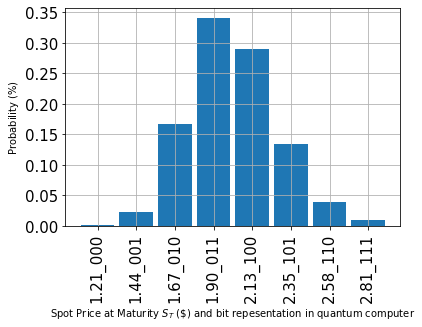
\includegraphics[width=0.5\linewidth]{images/probability.png}
  \end{center}
  \caption{The distinct log-normal distribution (eq. \ref{eq:lognormal}), with $\mu=(r-0.5\cdot \sigma^2)\cdot T + \log(S_0)$, $\sigma_{\text{dist}}=\sigma \cdot \sqrt{T}$ and as lower $l$ and highest $h$ value we used the 3 standard deviation. As x value the classical value is shown and the corresponding qubit state which are representing the number in our quantum computer.}
  \label{fig:E_log-normal}
\end{figure}

The equation of the European Payoff function is this
\begin{align}
    F(S(T)) = \max\{0, S(T) - K\} \label{eq:E_example_european}
\end{align}
and creates the result shown in figure \ref{fig:E_payoff_function}.
\begin{figure}[H]
  \begin{center}
    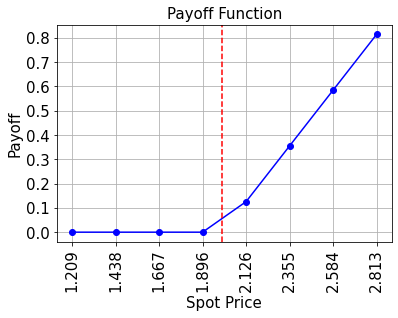
\includegraphics[width=0.5\linewidth]{images/payoff_european.png}
  \end{center}
  \caption{Here the value of the payoff function is shown. The breakpoints are set to $[0, 2.126]$ or $[\ket{000}, \ket{100}]$ thanks to ceil operation described in \ref{sec:MC_Payoff}}
  \label{fig:E_payoff_function}
\end{figure}

With this values we created our breakpoints, slopes and offsets. Important to know is that for our slope at breakpoint 1 we have to subtract slope(0), because the qubit already did a rotation for slope(0), the same for the offset. So we get this breakpoints, slopes and offsets, where we used $b_{\text{classic}} = [0, S_T ]$
\begin{align}
    br &= \frac{b_{\text{classic}}-l}{h-l} \cdot (2^{n}-1) \nonumber \\
    &= [0.0, 3.45206590600975] \nonumber \\
    \text{slopes}_\text{temp} &= [0, \pi c\frac{h-l}{2\cdot (f(i)_\text{max}-f(i)_\text{min}) \cdot(2^{n}-1)}] \nonumber \\
    \text{slopes}(b) &= \text{slopes}_\text{temp}(b) - \sum_{i=0}^{b-1} \text{slopes}(i) \nonumber \\
     &= [0.0,         0.22136774] \nonumber \\
    \text{offsets}_\text{temp} &= - \frac{\pi c^2}{2\cdot (f(i)_\text{max}-f(i)_\text{min})} \nonumber \\
    \text{offsets}(b) &= \text{offsets}_\text{temp} - \text{slopes}_\text{temp}(b) \cdot br(b) - \sum_{i=0}^{b-1} \text{offsets}(i) \nonumber \\
    &= [ 1.17809725, -0.76417604] \nonumber
\end{align}

This values then result in the circuit displayed in figure \ref{fig:E_model_payoff_function} and a probability distribution shown in figure \ref{fig:E_probability_estimate}
 
\begin{figure}[H]
  \begin{center}
    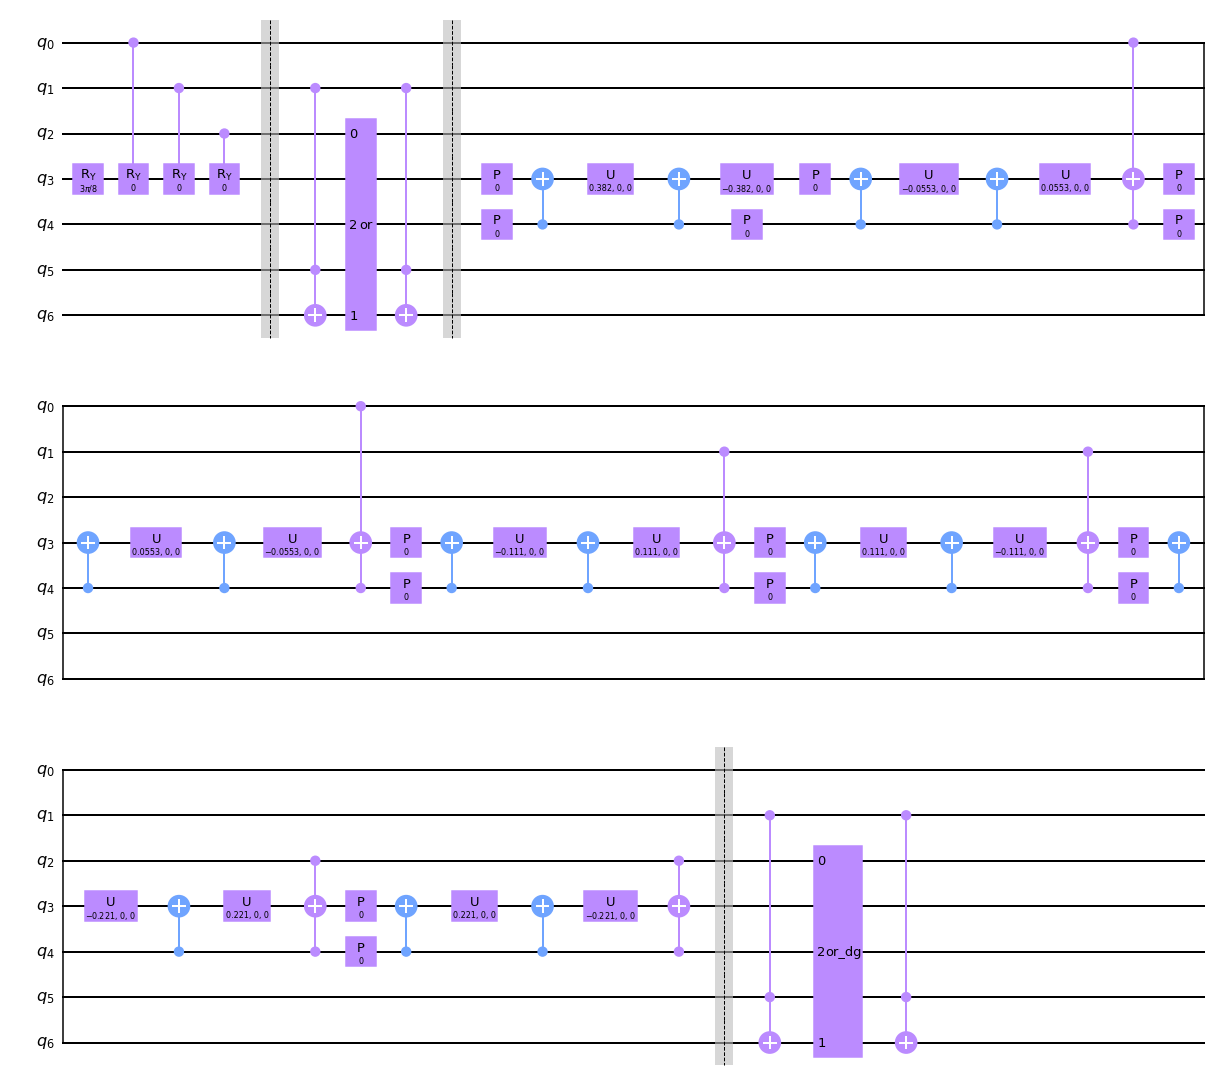
\includegraphics[width=\linewidth]{images/model.png}
  \end{center}
  \caption{The output of the circuit for the payoff function. The image of the circuit was generated by qiskit.\cite{Qiskit}. The circuit is divided in four sections. The first section is the $Y$-Rotation for the first breakpoint. The second section is then the greater or equal operation for the second breakpoint. The next section is then the rotation for the second breakpoint, here it good to see that the compare qubit is used to decide if the rotation should be executed or not. The last section is now the inverse of the second section.}
  \label{fig:E_model_payoff_function}
\end{figure}

 \begin{figure}[H]
  \begin{center}
    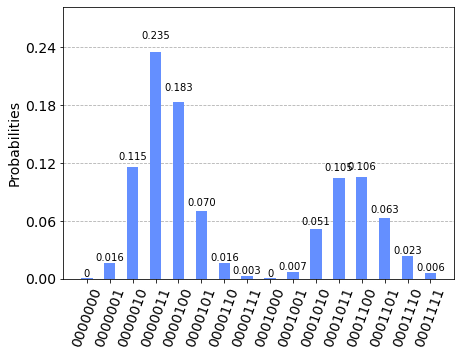
\includegraphics[width=0.5\linewidth]{images/probability_estimate.png}
  \end{center}
  \caption{The output after applying the payoff function to our circuit.}
  \label{fig:E_probability_estimate}
\end{figure}

The Grover Operator $\mathcal{Q}=AS_0A^\dagger S_{\psi_1}$ can now be used for the Phase Estimation Part of Amplitude Estimation. 

For European Call Options the $A$-gate of the Grover Operator is the circuit shown in figure $\ref{fig:E_model_payoff_function}$, $A^{\dagger}$ is simply the complex conjugate of $A$. $S_0$ is realized by a bit-flip of the objective qubit sandwiched by H-gates. The objective qubit is qubit 3 in our case, since thanks to the qubit saving implementation of $max$ function in \ref{fig:PF_max} a second ancilla qubit for A-gate is not needed.$S_{\psi_1} &= 1-2\ket{\psi_1}\ket{0}\bra{\psi_1}\bra{0}$ is implemented using $2\ket{\psi_1}\ket{0}\bra{\psi_1}\bra{0}-1$ and a global phase bit, since the negative form can easily be implemented by using multi-controlled Z-gates sandwiched by X-gates on the target qubit. The global phase has no effect on Grovers algorithm in general. The Grover is shown in figure \ref{fig:grover}

 \begin{figure}[H]
  \begin{center}
    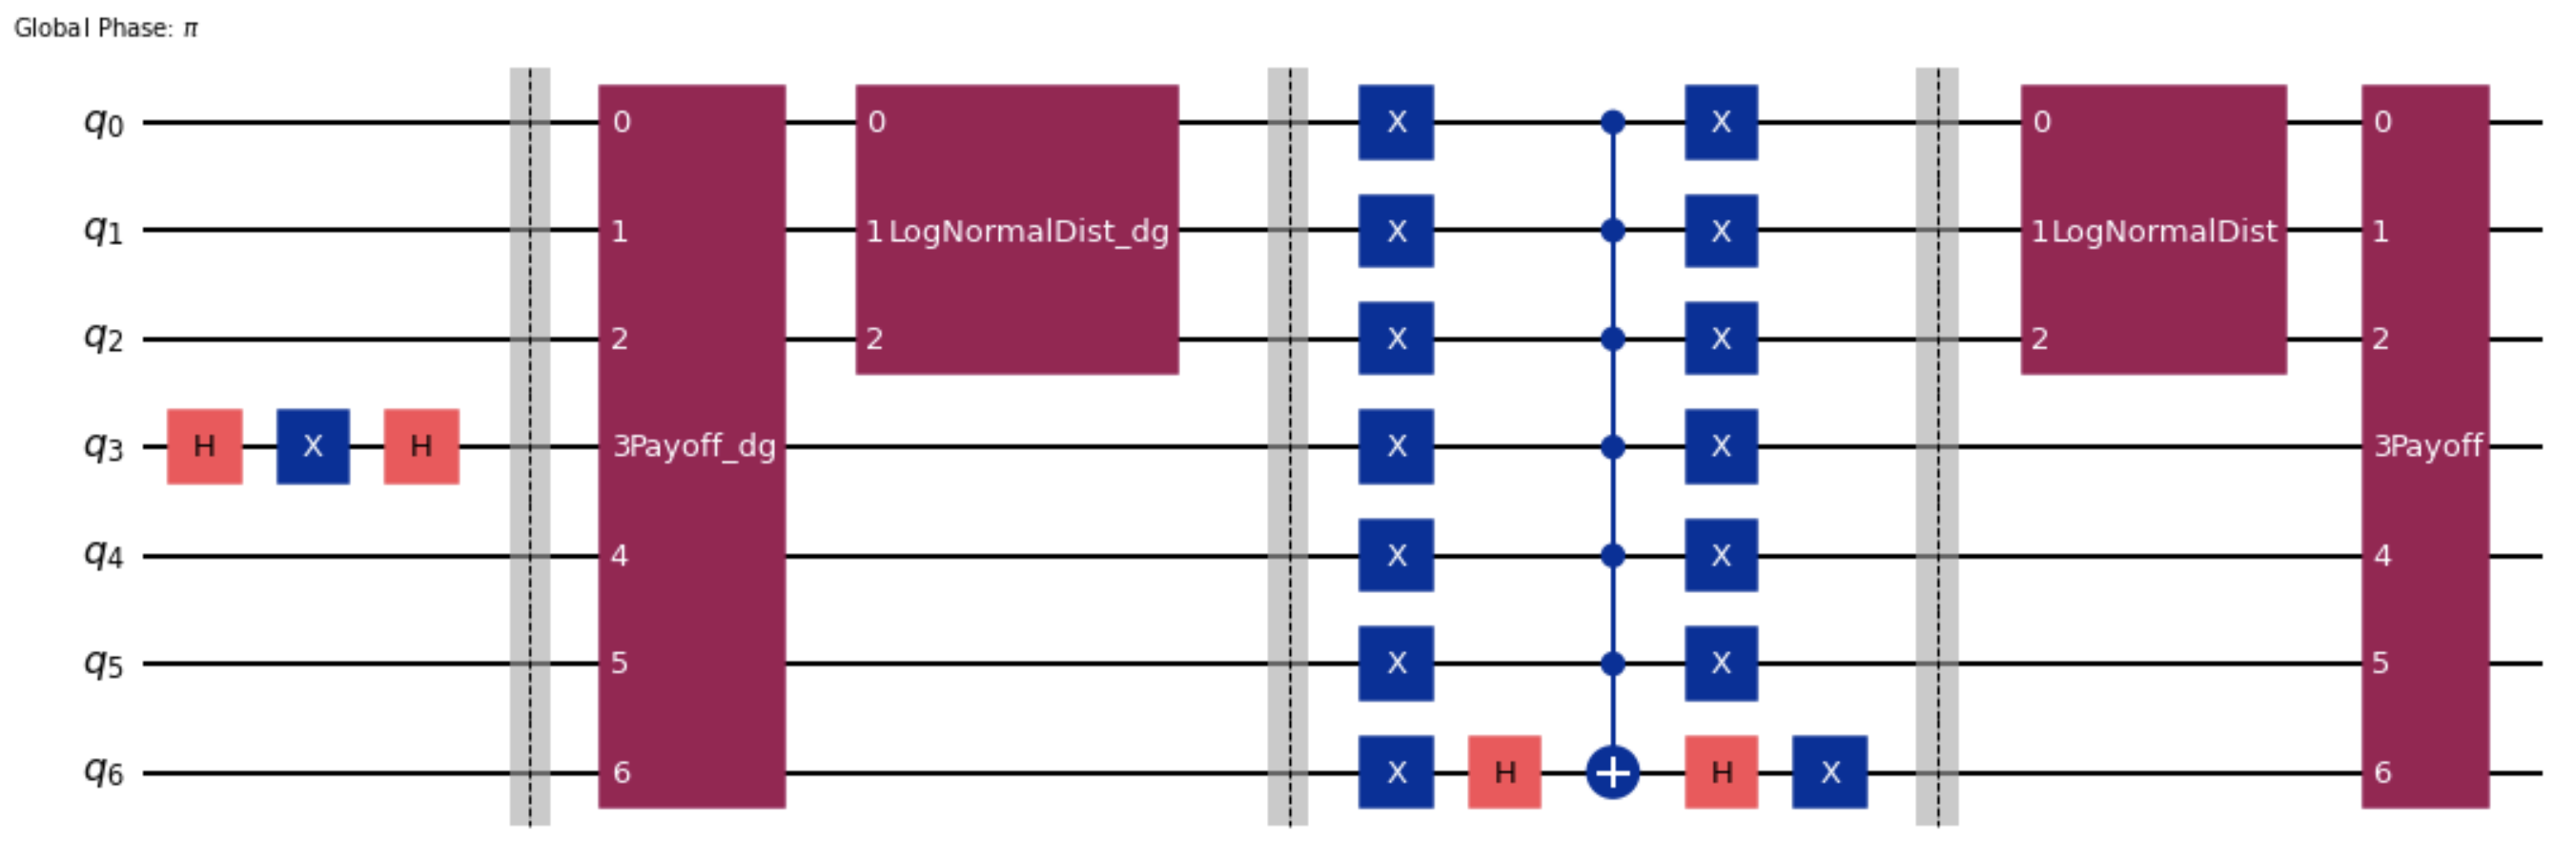
\includegraphics[width=\linewidth]{images/grover.png}
  \end{center}
  \caption{The Grover-operator. $S_0$ is a bit-flip implemented by a X-gate sandwiched by H-gates. $A$, $A^{\dagger}$ is the circuit and its complex-conjugate shown in figure $\ref{fig:E_model_payoff_function}$.\\
  $S_{\psi_1} &= 1-2\ket{\psi_1}\ket{0}\bra{\psi_1}\bra{0}$ is implemented using $2\ket{\psi_1}\ket{0}\bra{\psi_1}\bra{0}-1$ and a global phase bit.}
  \label{fig:grover}
\end{figure}

The Grover-operator can than be applied to the first register $\ket{i}$ controlled by a second evaluation register $\ket{m}$. See figure \ref{fig:qgan} for a schematic overview.\\

 \begin{figure}[H]
  \begin{center}
    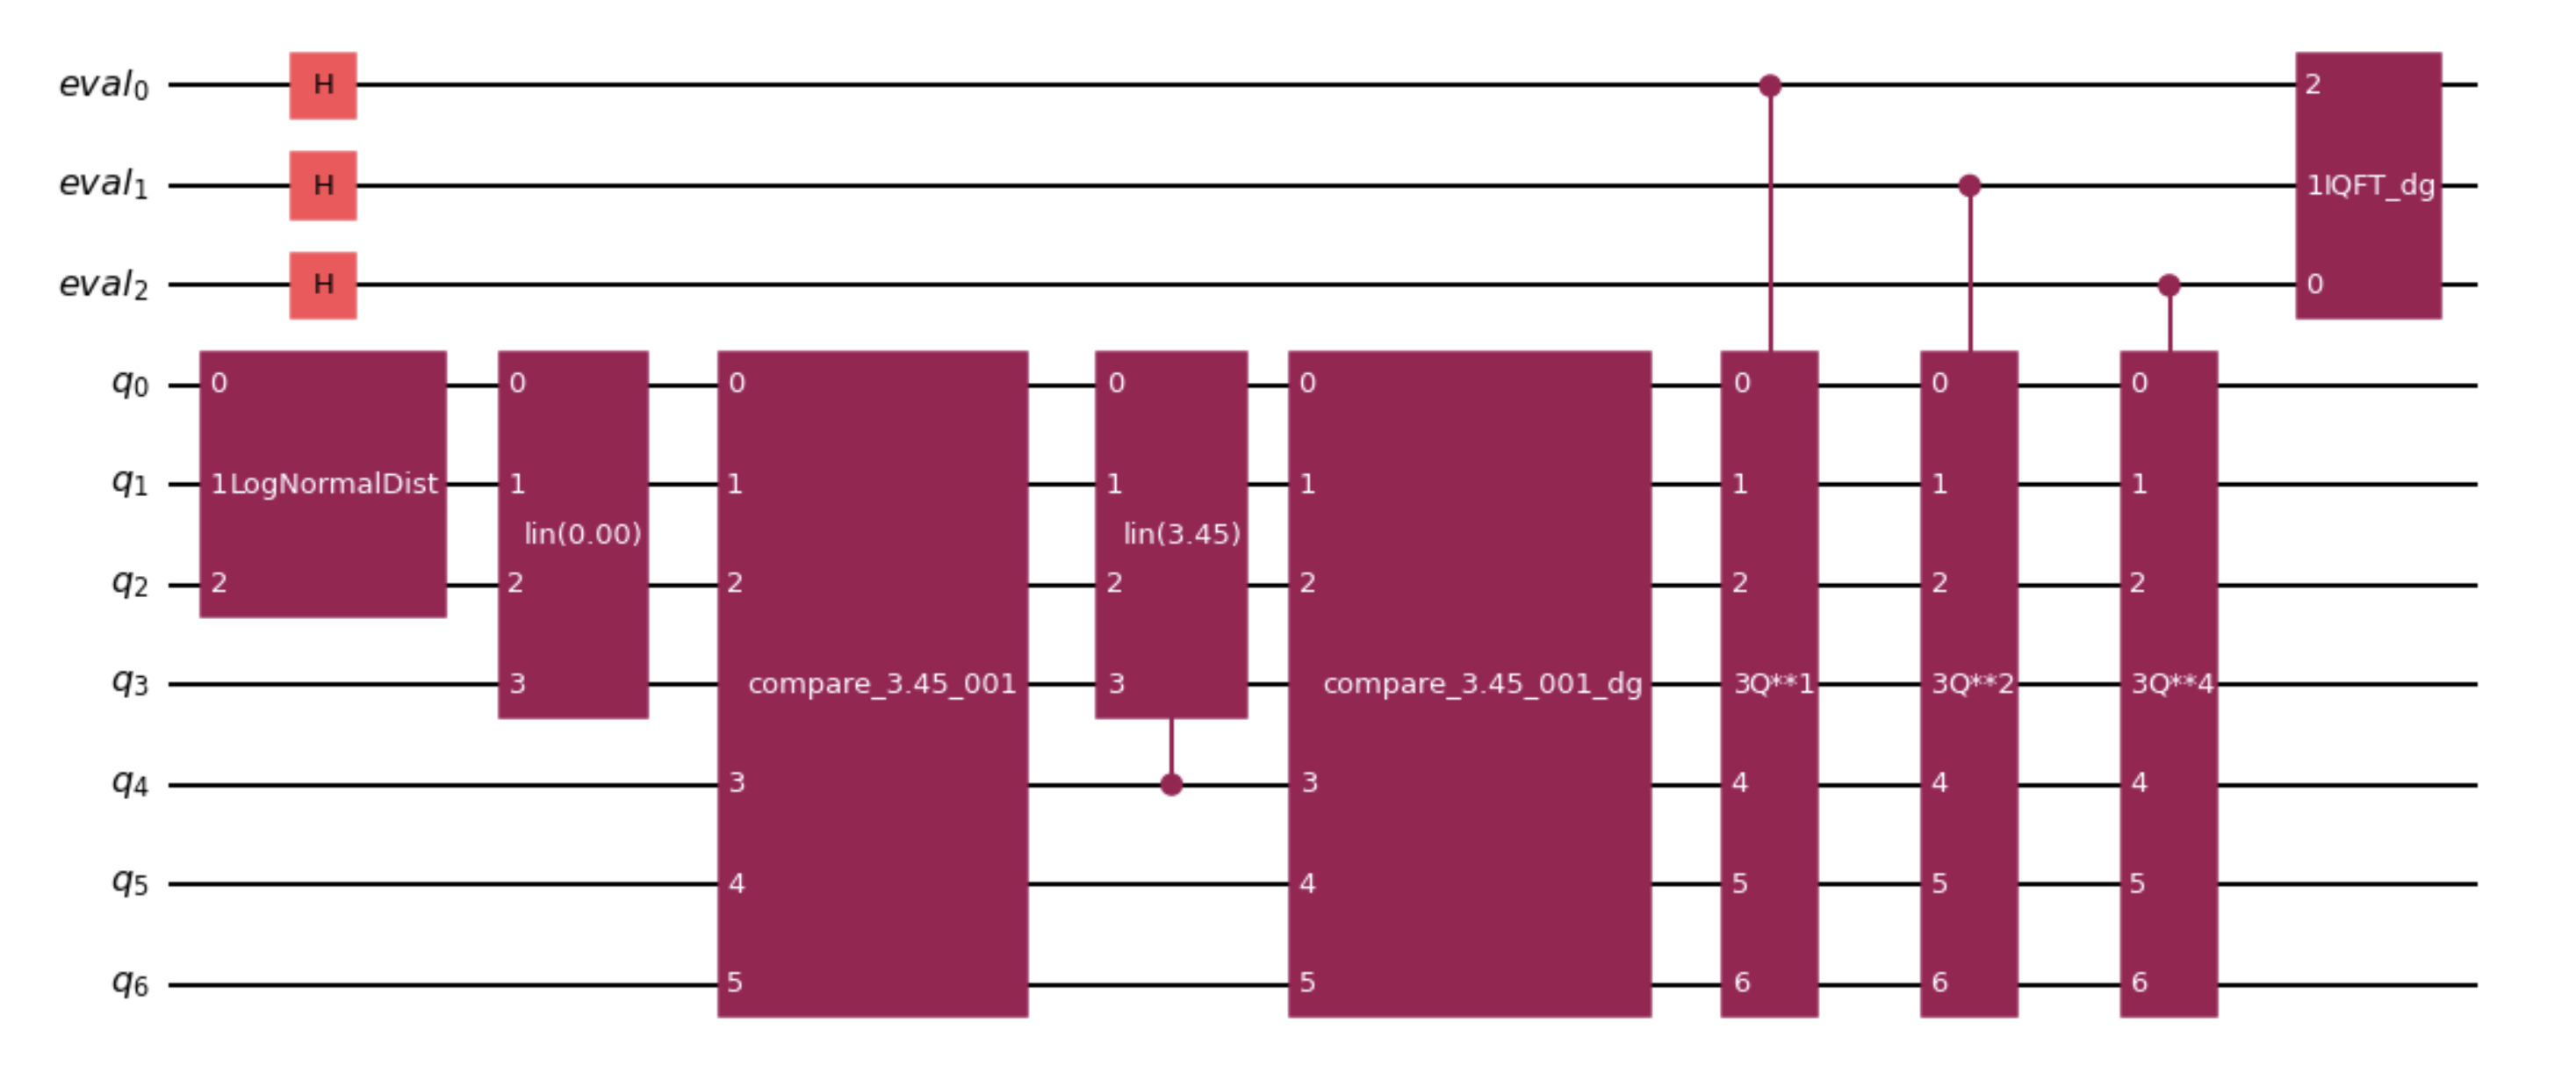
\includegraphics[width=\linewidth]{images/combinedCircuit.png}
  \end{center}
  \caption{The combined circuit. Note that the objective qubit here is qubit 3. Evaluation qubits are chosen for pragmatical reasons. For results a register consisting of seven qubits have been used.}
  \label{fig:combinedCircuit}
\end{figure}
The combined Circuit is displayed in figure $\ref{fig:combinedCircuit}$. For the obtained results, i.e. the estimate of Amplitude Estimation seven qubits in the evaluation register have been used. Measuring all qubits in the evaluation register gives the following result:
\begin{align}
    &\text{Exact Value: } &0.1133\\
    &\text{Estimated Value: } &0.1061\\
    &\text{95 Percent Confidence interval:	} &[0.1157, 0.1209]
\end{align}
Therefore the estimated value is close to the exact value. One problem here is that the estimated value does not lie within the confidence interval.
Note that the estimated value is the mean of applying eq. $\ref{eq:estimate_a}$ to the results of amplitude estimation. Additionally a post processing has been added in order to map from $[0,1]$ to the domain of stock prices. It is possible to apply a maximum likelihood estimator to the estimated value: 
\begin{equation}
    \text{MLE estimator value: } 0.1189.
\end{equation}
The value of the MLE estimator vaue is slightly better than the value of the ordinary estimator. Furthermore it lies within the confidence interval which is not the case for the estimated value.  
\\
 \begin{figure}[H]
  \begin{center}
    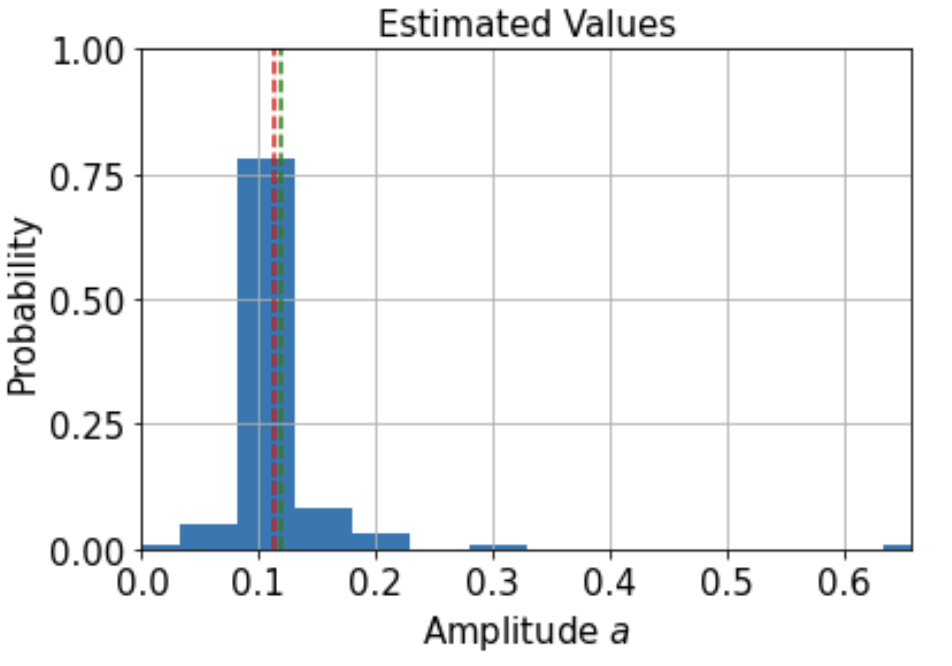
\includegraphics[width=\linewidth]{images/resultAE.png}
  \end{center}
  \caption{Results of Canonical AE. Red dotted line show the exact value. Green line is the MLE estimator value. }
  \label{fig:resultAE}
\end{figure}
When we now execute the same Circuit using Iterative Amplitude Estimation \cite{Grinko_2021} from qiskit we get the following results:
\begin{align}
    &\text{Exact Value: } &0.1133\\
    &\text{Estimated Value: } &0.1203\\
    &\text{95 Percent Confidence interval:	} &[0.1153, 0.1254]
\end{align}
Which is comparable to the values from Canonical Amplitude Estimation but comes with a lower cost, since Iterative Amplitude Estimation estimates the amplitude wihtout the usage of Phase Estimation and therefore with less qubits and gates.
\bibliography{./refs}
\section{Outlook and Conclusion}
In this report, we worked on reproducing the work of the paper \cite{1905.02666}. When we compare our result we get with the quantum computer and compare it with the result of the exact value we are  close to the exact result. But do not fit into the confidence interval unless a MLE estimation is used.\\
After investigating these problems we can apply Amplitude Estimation to even more complicated options types like path dependent once. Also generic functions can be fitted with piece-wise linear function and more research can be done on how to use the fitted linear functions in Amplitude Estimation. 
\bibliography{./refs}

\bibliography{refs}
\end{document}